\subsection{Ethylene pyrolysis in a flow reactor}
The PFR model was used to simulate\footnote{\href{https://github.com/mohammadadib-cu/omnisoot-cv/tree/main/examples/plug_flow/sectional}{https://github.com/mohammadadib-cu/omnisoot-cv/tree/main/examples/plug\_flow/sectional}} the pyrolysis of 0.6\% $\mathrm{C_2H_4}$-$\mathrm{N_2}$ in a 1.4 m long, and 16 mm diameter flow reactor. Figure~\ref{fig:pfr_temp} shows the axial temperature profile used in the simulations. The maximum temperature, $\mathrm{T_{max}} = 1673$ K, was imposed on the model based on thermocouple measurements reported by~\citet{mei2019quantitative} for various flow rates along the reactor centerline. The temperature increases from 300 K at the reactor inlet to the hot zone, where it reaches a value within 10\% of $\mathrm{T_{max}}$. The length of the hot zone varies with flow rate due to advection, ranging from 0.71 m at $\mathrm{Q}=8$ L/min to 0.76 m at $\mathrm{Q}=12$ L/min. Near the reactor outlet, the temperature drops to approximately 650 K.

The inception and PAH adsorption adjustment factors were varied to match the predicted PSD with Scanning Mobility Particle Sizer
(SMPS) measurements conducted on centerline at the reactor exit for the flow rates of 8, 11, and 12 L/min~\citep{mei2019quantitative}, as shown in Figure~\ref{fig:pfr_psd}. The parametric analysis revealed that each inception model requires a unique set of adjustment factors to minimize the PSD prediction error across different flow rates. The KAUST mechanism~\citep{wang2013pah} was used to describe gas-phase chemistry, as it provided better agreement with the measured PSDs than the Caltech mechanism, shown in Figure~\ref{fig:pfr_psd_caltech}.

A bimodal size distribution can be observed for $\mathrm{Q}=8$ L/min (Figure~\ref{fig:pfr_psd}a) that was attributed to the continuous inception~\citep{zhao2003measurement}. The comparison of simulations with measurements reveals different temperature dependence of inception models. Irreversible Dimerization and Dimer Coalescence models capture the bimodality of PSD in good agreement with the measurements, but the other two models predict a nearly unimodal PSD. Specifically, the number concentration of the first section is lower by more than three orders of magnitude for the Reactive Dimerization and E-Bridge Modified models indicating the lack of active inception at the sampling location due to the temperature drops near the end of reactor that suppresses soot inception.

All inception models capture the disappearance of the PSD shoulder at flow rates of 11 and 12 L/min. In these cases, the shorter particle residence time limits coagulation, preventing formation of a second peak. However, Reactive Dimerization and E-Bridge Modified models still underpredict the number concentration of nascent particles by approximately one order of magnitude compared to the irreversible models (Irreversible Dimerization and Dimer Coalescence).




\begin{figure}[H]
	\centering
	\begin{tikzpicture}
		\draw (0, 0) node[inner sep=0] 	{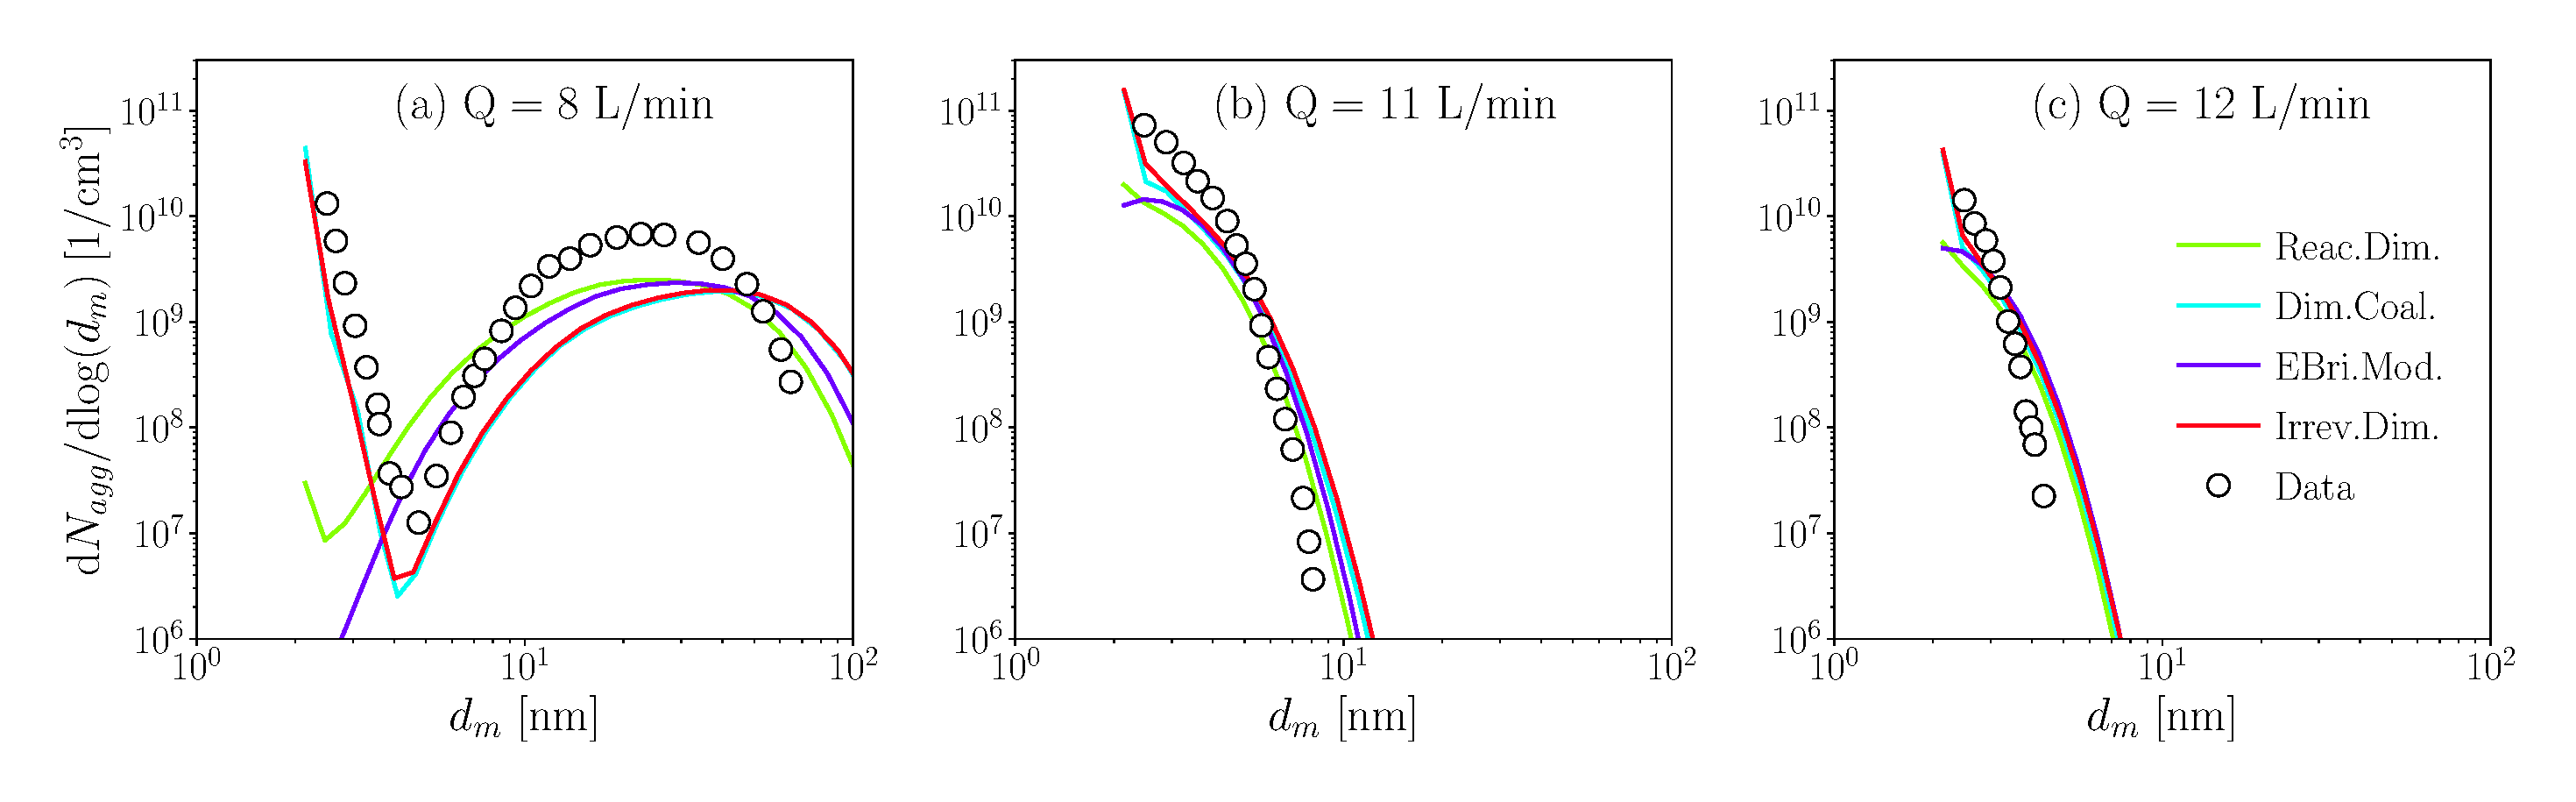
\includegraphics[width=1\textwidth]{Figures/Results/PFR/PSD_diffQ.pdf}};
		\draw (6.63, -0.51) node {\scriptsize{\cite{mei2019quantitative}}};
	\end{tikzpicture}
	\caption{The particle size distribution at the end of PFR for $\mathrm{Q}=8$ (a), 11 (b), and 12 L/min (c) obtained using KAUST mechanism, SPBM and different inception models calibrated to match the predictions with measurement~\citep{mei2019quantitative}.}
	\label{fig:pfr_psd} 
\end{figure}

Figure~\ref{fig:pfr_Nagg} presents the axial evolution of $N_{agg}$. All inception models predict nearly the same $N_{agg}$ up to $z \approx 1.1$ m, corresponding to the end of the hot zone. Beyond this point, $N_{agg}$ continues to increase for the Irreversible Dimerization and Dimer Coalescence models, which allows soot inception to proceed in cooler downstream regions. These models agree well with experimental data at 8 and 11 L/min but tend to overpredict $N_{agg}$ at 12 L/min.

As shown in Figure~\ref{fig:pfr_Iinc}, soot inception flux rises sharply as the gas enters the hot zone. The axial location where the flux exceeds $10^7~\mathrm{cm^{-3}~s^{-1}}$ is similar across all inception models, as it is primarily determined by PAH chemistry. However, this location shifts downstream with increasing flow rate due to reduced residence time. Within the hot zone, differences among the inception models are minimal. Outside the hot zone, Irreversible Dimerization and Dimer Coalescence models maintain high inception flux, while Reactive Dimerization and E-Bridge Modified models predict a rapid decrease of more than three orders of magnitude due to cooling. Figure~\ref{fig:pfr_cmap} demonstrates the contribution of each pathway to total carbon mass of soot along the reactor, which elucidates the link between particle morphology and the balance of inception and surface growth. The relative contribution of inception decreases from 100\% to less than 5\% by $z=1.1$ m for all inception models leading to a gradual increase in $d_p$ and $d_m$. Irreversible Dimerization and Dimer Coalescence models predict an increase in the contribution of inception beyond $z>1.1$~m resulting in the decline of $d_p$ while Reactive Dimerization and E-Bridge Modified models predict a nearly constant $d_p$ close to 5 nm. The final increase in $d_m$ beyond the end of the hot zone near $z = 1.1$~nm is more pronounced for the Reactive Dimerization and E-Bridge Modified models. This is because the inception rate (Figure~\ref{fig:pfr_Iinc}) and surface growth rate (Figure~\ref{fig:pfr_surfacegrowth}) rapidly decrease in these models, and soot morphology becomes primarily governed by coagulation, which conserves $d_p$ and increases $d_m$.


%fig:pfr_surfacegrowth

\begin{figure}[H]
	\centering
	\begin{tikzpicture}
		\draw (0, 0) node[inner sep=0] 	{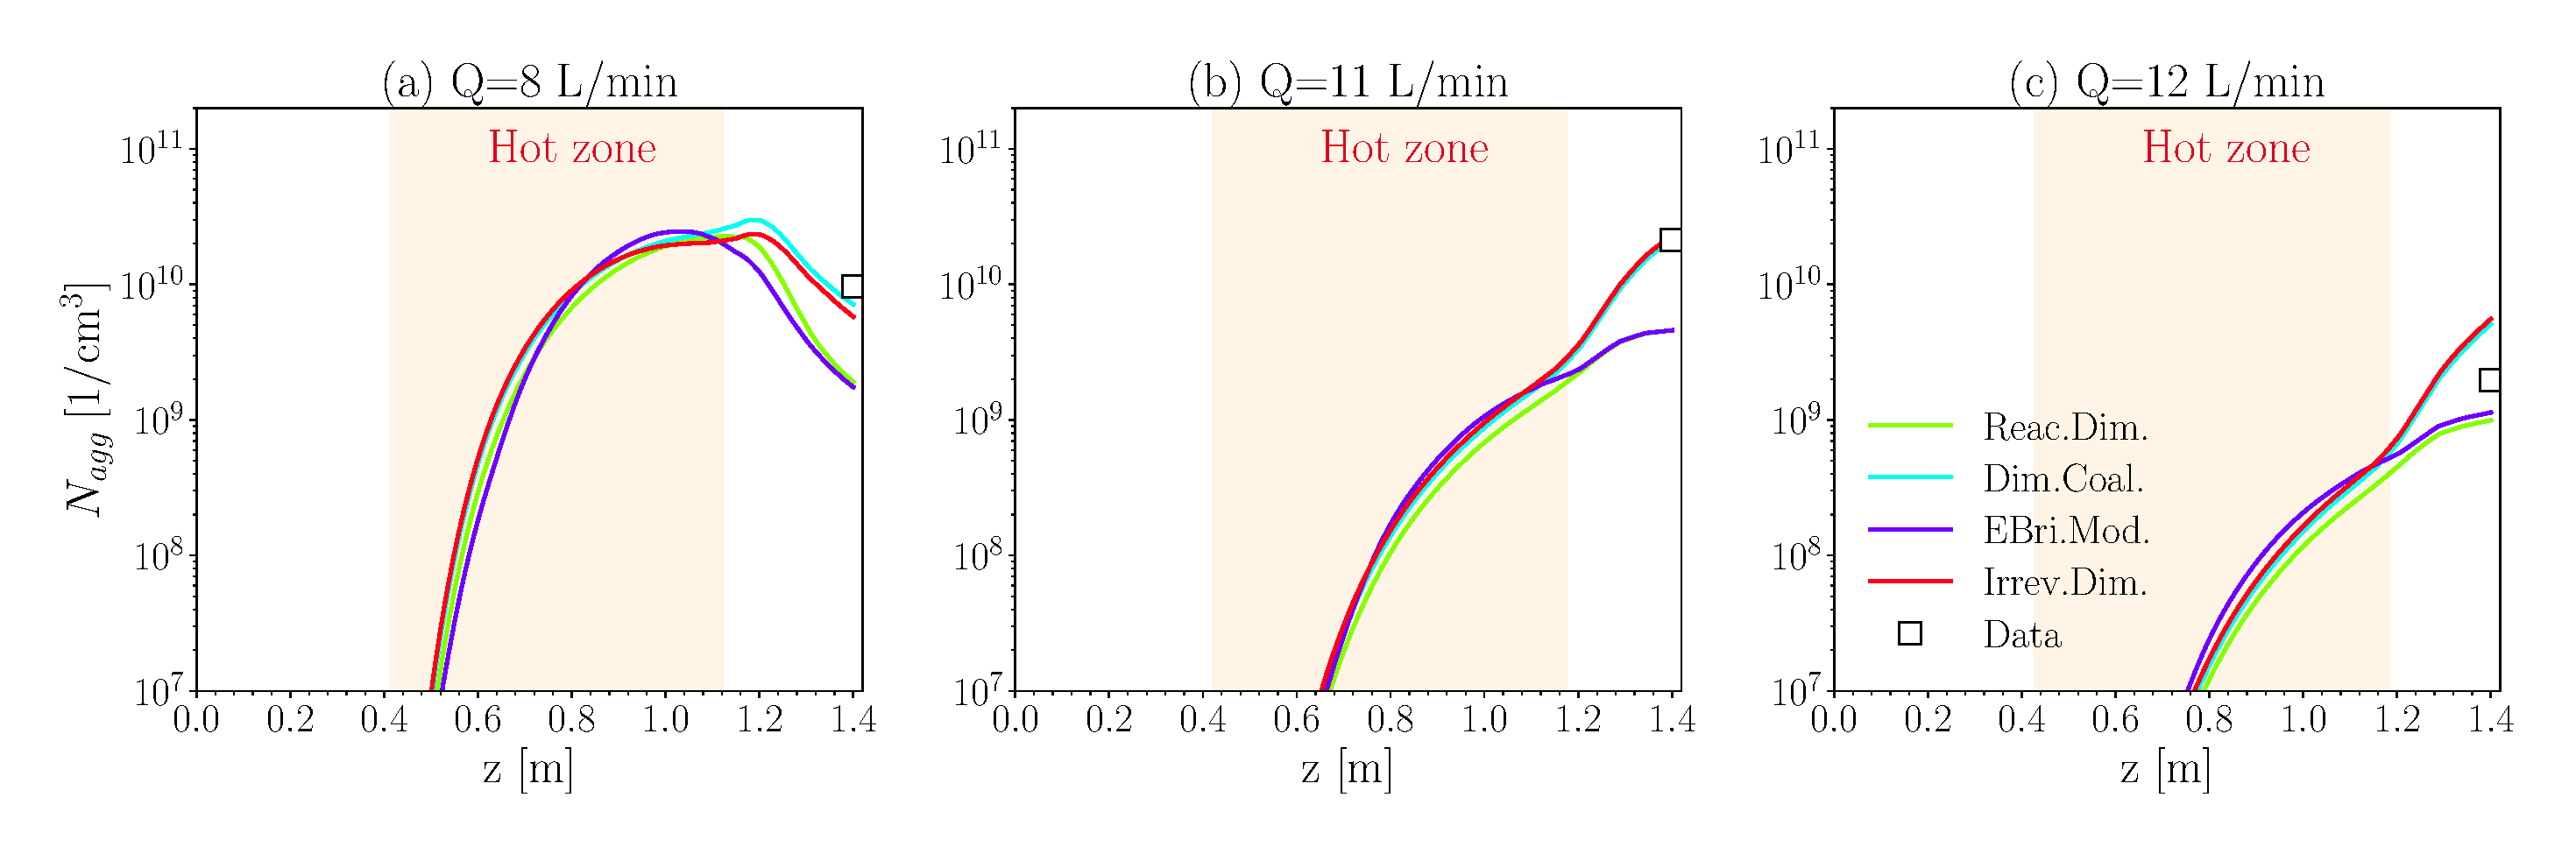
\includegraphics[width=1\textwidth]{Figures/Results/PFR/N_agg.pdf}};
		\draw (4.85, -1.25) node {\tiny{\cite{mei2019quantitative}}};
	\end{tikzpicture}
	\caption{The total number of agglomerates along the PFR for $\mathrm{Q}=8$ (a), 11 (b), and 12 L/min (c) obtained using KAUST mechanism, SPBM and different inception models compared with data~\citep{mei2019quantitative}. The yellow area represents the hot zone ($\mathrm{T}>0.9\mathrm{T_{max}}$).}
	\label{fig:pfr_Nagg} 
\end{figure}

\begin{figure}[H]
	\centering
	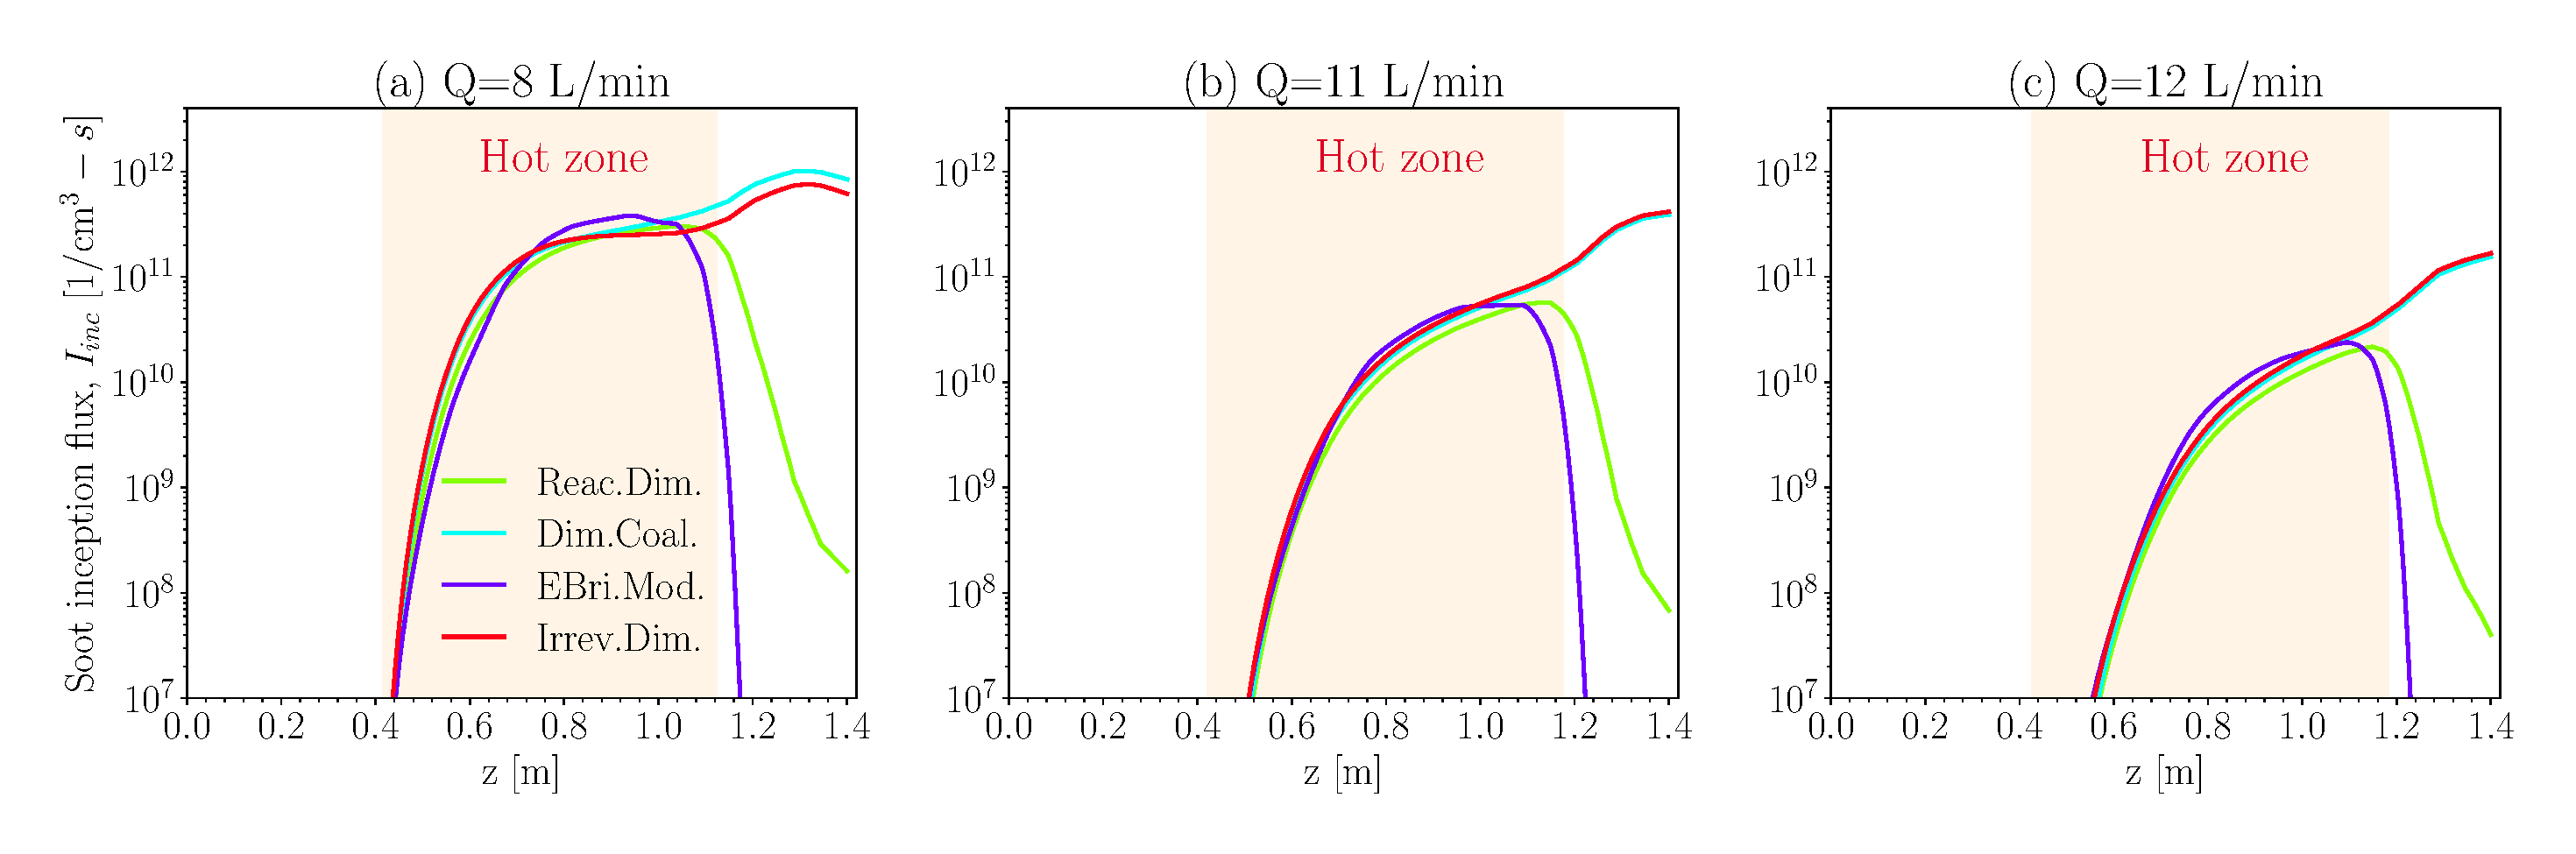
\includegraphics[width=1\textwidth]{Figures/Results/PFR/inception.pdf}
	\caption{The soot inception flux along the PFR for $\mathrm{Q}=8$ (a), 11 (b), and 12 L/min (c) obtained using KAUST mechanism, SPBM and different inception models. The yellow area represents the hot zone ($\mathrm{T}>0.9\mathrm{T_{max}}$).}
	\label{fig:pfr_Iinc} 
\end{figure}


\begin{figure}[H]
	\centering
	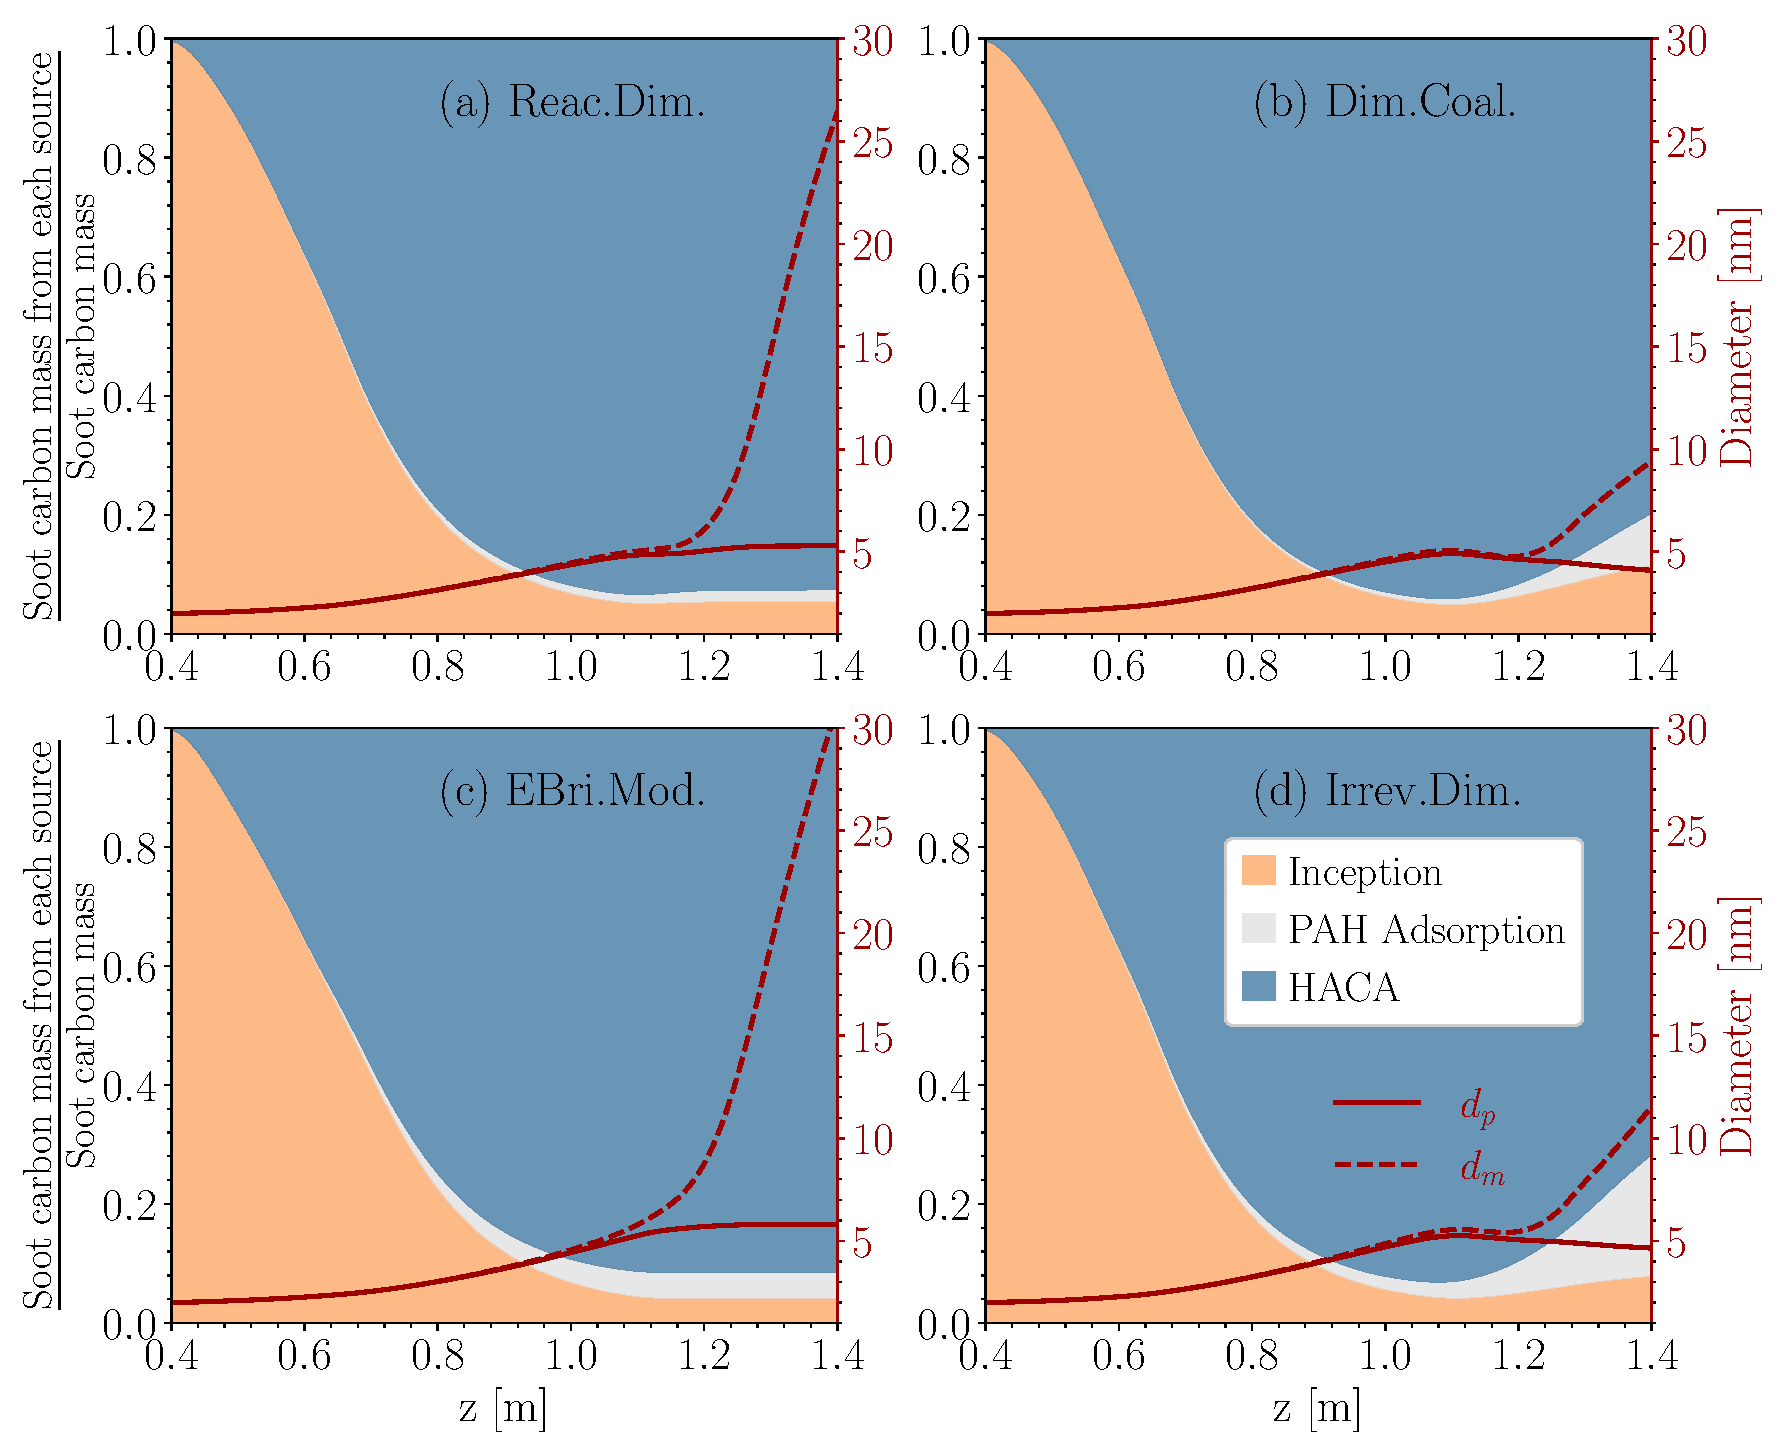
\includegraphics[width=0.8\textwidth]{Figures/Results/PFR/C_tot_distmap.pdf}
	\caption{The soot carbon mass from inception, PAH adsorption and HACA normalized by total soot carbon mass for $\mathrm{Q}=8$ L/min along with $d_p$ and $d_m$ obtained using KAUST mechanism, SPBM and different inception models.}
	\label{fig:pfr_cmap} 
\end{figure}